\documentclass[11pt]{article}
\usepackage{amsmath,amssymb, amsthm, marvosym, permute, extsizes}
\usepackage{siunitx, graphicx, float, enumitem, adjustbox, hyperref, bm}
\usepackage{microtype, dsfont}
\usepackage[normalem]{ulem}
\usepackage[T1]{fontenc}
\usepackage[utf8]{inputenc}
\usepackage{lmodern}
\usepackage[T1]{fontenc}
\usepackage[a4paper,margin=2.5cm]{geometry}
\usepackage[icelandic]{babel}
\usepackage{tikz}
\newcommand{\explain}[2]{\underbrace{#1}_\textrm{$#2$}}

\usepackage{minted}

\title{\vspace{-2ex}Heimadæmi 9\\ \vspace{0.2cm} \large Töluleg Greining\vspace{-2ex}}
\author{Emil Gauti Friðriksson}
\begin{document}
\maketitle
\section*{Dæmi 1}
Develop a second-order method for approximationg $f'(x)$ that uses the data $f(x-2h),f(x)$ and $f(x+3h)$ only.
\subsection*{Svar}
Byrjum á því að rita niður Taylor nálganirnar fyrir $f(x+3h)$ og $f(x-2h)$
\begin{align*}
f(x+3h) &= f(x) + 3hf'(x) + \frac{(3h)^2}{2}f''(c)\\
f(x-2h) &= f(x) - 2hf'(x) + \frac{(-2h)^2}{2}f''(c)
\end{align*}
skilgreinum svo fallið $g(x) = af(x+3h) + bf(x-2h) + cf(x)$ þar sem $a,b,c$ eru fastar sem ráðast af eftirfarandi:
\begin{align*}
g(x) = (a+b+c)f(x) + (3a-2b)hf'(x) + (9a+4b)\frac{h^2}{2}f''(x)
\end{align*}
en við viljum gera nálgun á $f'(x)$ svo við viljum láta $a+b+c = 0$, $3a-2b = 1$ og $9a+4b = 0$, fáum úr þessu einfalt jöfnuhneppi sem hefur lausnirnar $a=\frac{2}{15}$, $b=\frac{-3}{10} $ og $c=\frac 16$. Stingum þessu aftur inn í $f'(x) = g(x)/h = (af(x+3h) + bf(x-2h) + cf(x))/h$ og fáum:
\begin{align*}
f'(x) 	&= \frac{\frac{2}{15}f(x+3h)-\frac{3}{10}f(x-2h) + \frac{1}{6} f(x) }{h} - h^2f'''(c)\\
		&= \frac{4f(x+3h)-5f(x)-9f(x-2h)}{30h} - h^2f'''(c)
\end{align*}



\section*{Dæmi 2}
Hvað gerir eftirfarandi forrit? Keyrið það og túlkið niðurstöðuna. Gefið tvær ástæður fyrir því af hverju afleiðunálganir af lágu stigi eru einstaklega óheppilegar þegar nálga á afleiðu falls á heilu bili.

\begin{minted}{matlab}
 function daemi1(a)
 p=-20:0;
 f=@(x) sin(x);
 df=@(x) cos(x);
 for i=1:length(p)
 h=10^p(i);
 err1(i)=(f(a+h) - f(a-h))/(2*h)-df(a);
 err2(i)=(f(a+h) - f(a))/h-df(a);
 h=2*h;
 err3(i)=(f(a-h)-8*f(a-h/2)+8*f(a+h/2) - f(a+h))/(6*h)-df(a);
 end
 hold on
 plot(p,log10(abs(err1)),'b')
 plot(p,log10(abs(err2)),'r')
 plot(p,log10(abs(err3)),'g')
 legend('err1', 'err2', 'err3')
 end
\end{minted}
Forritið skilar eftirfarandi mynd fyrir skipunina \mintinline{matlab}{daemi1(3)}

\begin{figure}[H]
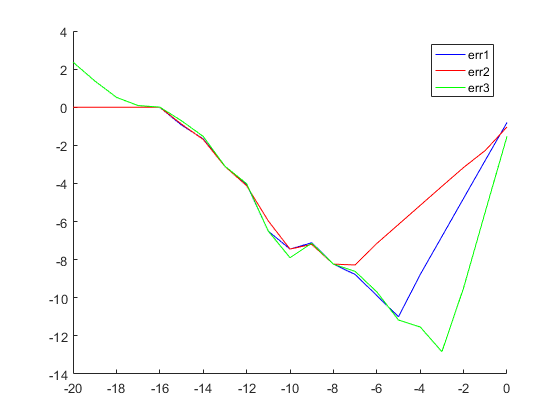
\includegraphics[scale=1]{mynd1.png}
\end{figure}
Hér sjáum við að ef við förum til hægri meðfram x-ás þá stækkar $h$, við erum að teikna upp logrann af skekkju þriggja nálganna fyrir afleiðu fallsins $\sin(x)$ með breytilegu $h$. Skekkjan er minnst þar sem grafið er sem lægst. Það sem er áhugavert við þetta er að skekkjan er furðulega há fyrir lítil gildi á $h$ en það má útskýra á tvennan veg:
\begin{enumerate}
\item Þegar deiling á sér stað þar sem nefnarinn er mjög lítil tala þá getur komið fram umtalsverð skekkja. Tölvan gerir nálgun í útreikningunum sem skilar stórri skekkju í lokasvarinu.
\item Þegar frádrátturinn á sér stað milli nálgunargildisins og raungildis getur komið fram skekkja ef tölurnar eru nánast þær sömu.
\end{enumerate}
Þess vegna fáum við minnstu skekkjuna þegar $h\approx 10^{-5}$


\newpage
\section*{Dæmi 3}
\textbf{(a)} Use the composite Trapezoid Rule with m = 16 and 32 panels to approximate the definite
integral. Compare with the correct integral and report the two errors.\\
$$\int_0^{2\,\sqrt[]{3}}\frac{1}{\sqrt[]{x^2+4}} dx $$

\textbf{(b)}
Apply the composite Simpson’s Rule to the integrals in previous problem. Use m = 16 and 32, and report errors.


\subsection*{Svar(a)}
Áður en við hefjumst handa skulum við finna rétta gildið á heildinu:\\
það er $I=\sinh^{-1}(\sqrt[]{3}) \approx 1.316958$
Notast var eftirfarandi forrit:
\begin{minted}{matlab}
f =@(x) 1/(x^2+4)^(0.5);
a = 0;
m=16;
b= 2*sqrt(3);
h = (b-a)/m;
sum = 0;
for i=1:m-1
    sum = sum + f(i*h);
end

heildi = h/2*(f(a)+f(b)+2*sum)
\end{minted}
sem skilar fyrir $m=16$:
\begin{minted}{matlab}
heildi = 1.316746488192236
\end{minted}
og hefur error: $|1.316746488192236 - I| = 2.114\cdot 10^{-4}$\\
og ef við notum $m=32$:
\begin{minted}{matlab}
heildi = 1.316905040381116
\end{minted}
og hefur error: $|1.316905040381116 - I| = 5.286\cdot 10^{-5}$


\subsection*{Svar(b)}
Notast var við eftirfarandi forrit:
\begin{minted}{matlab}
f =@(x) 1/(x^2+4)^(0.5);
a = 0;
m=16;
b= 2*sqrt(3);
h = (b-a)/(2*m);
sum = 0;
sum2 = 0;
for i=1:m
    sum = sum + f(2*i*h-h);
end
for j=1:m-1
    sum2 = sum2 + f(2*j*h);
end

heildi = h/3*(f(a)+f(b)+4*sum+2*sum2)
\end{minted}
sem skilar fyrir $m=16$:
\begin{minted}{matlab}
heildi = 1.316957891110743
\end{minted}
og hefur error $|1.316957891110743 - I| \approx 5.814\cdot 10^{-9}$\\
Athugum nú fyrir $m=32$:
\begin{minted}{matlab}
heildi = 1.316957896561761
\end{minted}
og hefur error $|1.316957896561761 - I| \approx 3.6301\cdot 10^{-10}$






\end{document}
